\documentclass[12pt]{article}
\usepackage{fancyhdr}
\usepackage[a4paper, margin=1.2in]{geometry} % Set page margins to

\usepackage{enumitem}
\usepackage{tikz}
\usepackage{amssymb}
\usepackage{adjustbox}
\usepackage{hyperref}
\usetikzlibrary{automata, positioning}

% Set up the page style
\pagestyle{fancy}
\fancyhf{}
\lhead{\courseName}
\rhead{\thepage}
%\fancyfoot[L]{\hrule\vspace{2pt}\studentInfo}

\newcommand{\defaultindent}{\setlength{\parindent}{1cm}}
% Define variables for course details and student information
\newcommand{\courseUniversity}{University of Colombo School of Computing}
\newcommand{\courseName}{SCS3203 Middleware Architecture}
\newcommand{\assignmentTitle}{Assignment 1}
\newcommand{\studentInfo}{
\begin{itemize}[label={}, noitemsep]
\item \hspace{5cm} Team KID\textsuperscript{2}S
\vspace*{0.5cm}
\item \hspace{3cm} 20000103 - D.A. Amarasinghe 
\item \hspace{3cm} 20001207 - K.K.S Nayanathara
\item \hspace{3cm} 20000723 - A.A.D Harshani
\item \hspace{3cm} 20000766 - P.A.I Heshan
\item \hspace{3cm} 20000804 - J.K.K.K. Jagoda
\end{itemize}
}

\begin{document}

% Title page
\begin{titlepage}
    \centering
    \vspace*{1cm}
    {\LARGE \courseUniversity \par}
    \vspace{1.5cm}
    {\Large \courseName \par}
    \vspace{1cm}
    {\Large \assignmentTitle \par}
    \vspace{2cm}
    {\large \studentInfo \par}
    \vfill
    {\large \today \par}
\end{titlepage}

% Reset page numbering
\pagenumbering{arabic}
\setcounter{page}{1}

% Answer sheet
\section*{Task 4}

%\begin{center}
\subsection*{Enhance the Architecture to Gain Improvement in Availability and Reliability\\}
%\end{center}

Our system's existing Pub/Sub application relies on just one server node, which has a big impact on its availability and dependability. We suggest a strong, distributed design to overcome this issue, ensuring increased fault tolerance and constant communication even in the event of server failure. A central broker serves as an intermediary between publishers and subscribers in the new architecture, which is built on a broker-based Pub/Sub paradigm. Copies of the broker are hosted by numerous server nodes, enabling redundancy and load balancing. The broker effectively transmits communications that publishers give to it to the right subscribers. We can eliminate the single point of failure by decentralizing the system and having numerous broker instances, ensuring continued communication even if one of the servers fails. To achieve high availability and data integrity, we can employ fault detection techniques and data replication across servers.\\

The proposed distributed design gives our current system a number of significant upgrades. The addition of several broker instances, in the first place, ensures fault tolerance and reduces the possibility of communication breakdown due to server failures. The demand is distributed equitably across the system since each server node hosting a broker may manage client connections and topic subscriptions. The implementation of asynchronous communication methods further improves the performance and responsiveness of our Pub/Sub system. Utilizing a load balancer also makes it possible to utilize resources effectively and avoid overloading particular nodes. We will be able to accomplish data redundancy and better resource usage by sharding topics and replicating broker state, which increases reliability. We can include monitoring and auto-scaling systems, enabling the system to automatically modify its capacity based on the load, to maintain the system's health and scalability. Overall, the distributed Pub/Sub architecture that is being suggested offers a reliable messaging system that can resist server outages and maintain constant user communication. \\

\begin{figure}[htbp]
    \centering
    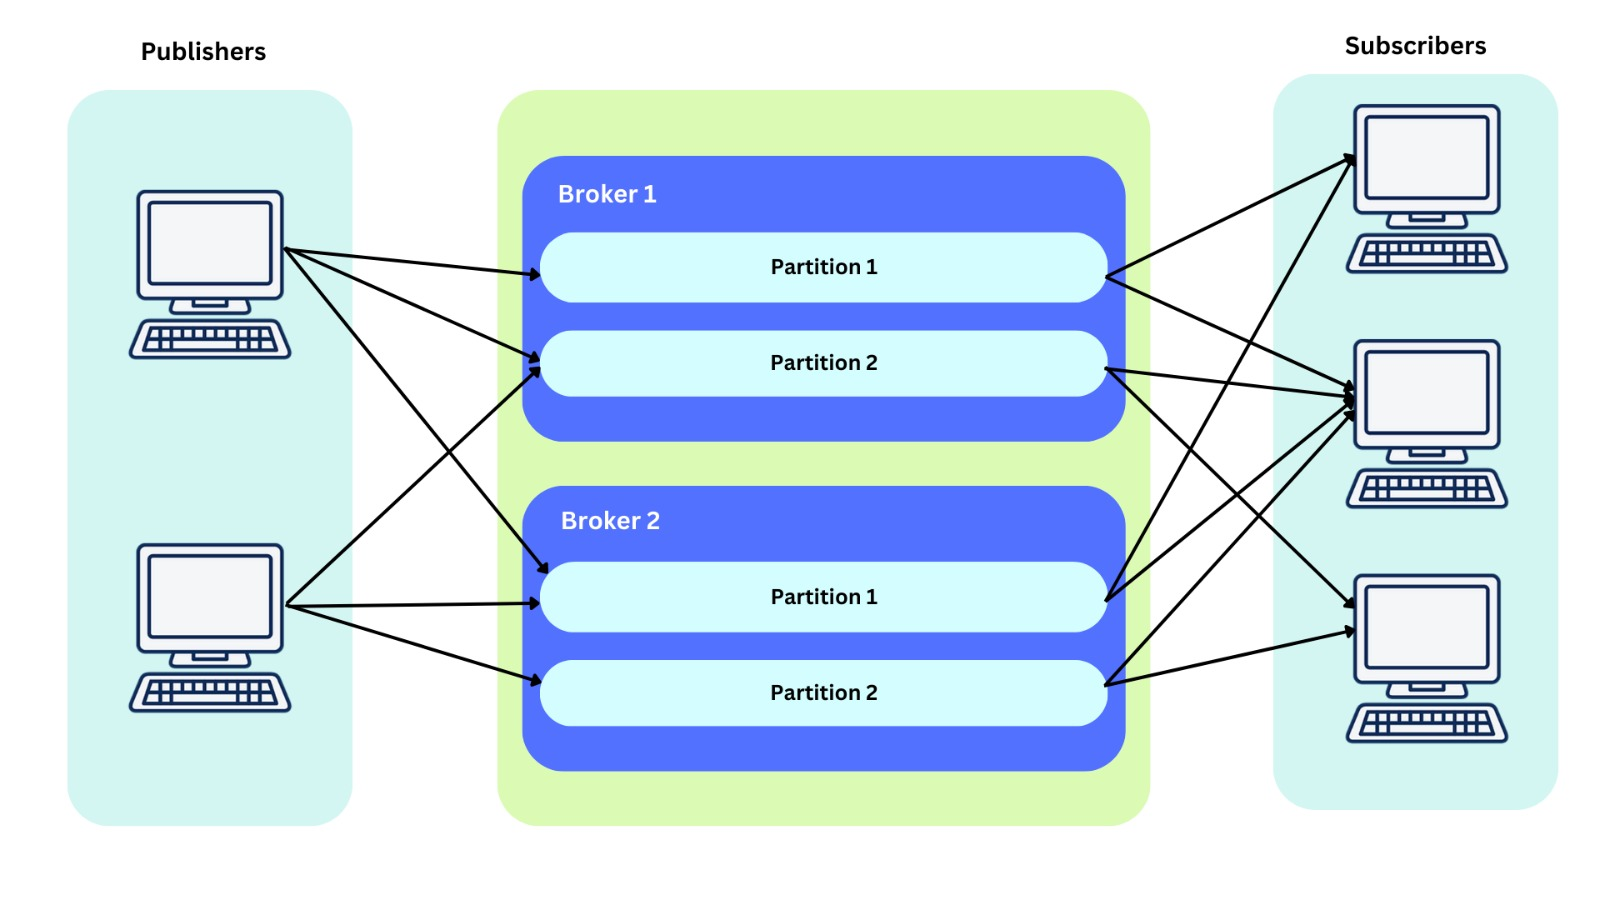
\includegraphics[width=\textwidth]{diagram.jpeg}
    \caption{Distributed pub-sub model \href{https://drive.google.com/file/d/1Fb0DC_PNNx6Xuwt2y6slLfDzqltXbMOb/view?usp=sharing}{\textcolor{blue}{link}}}
    \label{fig:sample}
\end{figure}

\noindent
GitHub Repository: \href{https://github.com/dinukaashan77/middleware_architecture.git}{\textcolor{blue}{https://github.com/dinukaashan77/middleware\_architecture.git}}

\end{document}
